\documentclass[12pt, a4paper]{article}

% CONFIGURACIÓN BÁSICA
\usepackage[spanish]{babel}
\usepackage[utf8]{inputenc}
\usepackage[T1]{fontenc}
\usepackage{lmodern}
\usepackage{csquotes}

% FORMATO Y DISEÑO
\usepackage{geometry}
\geometry{a4paper, margin=2.5cm, headheight=14pt}
\usepackage{fancyhdr}
\usepackage{setspace}
\onehalfspacing
\usepackage{enumitem}
\usepackage{graphicx}
\usepackage{float}
\usepackage{caption}

% MATEMÁTICAS Y SÍMBOLOS
\usepackage{amsmath}
\usepackage{amsfonts}
\usepackage{amssymb}

% CÓDIGO Y LISTADOS
\usepackage{listings}
\usepackage{xcolor}

% CONFIGURACION DEL YAML

\lstdefinelanguage{yaml}{
    keywords={},
    sensitive=false,
    comment=[l]{\#},
    morestring=[b]",
}

% ENLACES Y REFERENCIAS
\usepackage{hyperref}
\hypersetup{
    colorlinks=true,
    linkcolor=blue,
    filecolor=magenta,      
    urlcolor=cyan,
    pdftitle={Configuración de red Raspberry y VM},
}

% CONFIGURACIÓN DE LISTINGS
\lstset{
    basicstyle=\ttfamily\small,
    keywordstyle=\color{blue},
    stringstyle=\color{red},
    commentstyle=\color{green},
    showstringspaces=false,
    numbers=left,
    numberstyle=\tiny\color{gray},
    frame=single,
    breaklines=true,
    morekeywords={systemctl, journalctl, service, ip, sudo, qemu-system-x86_64, k3s, kubectl},
    inputencoding=utf8,
    extendedchars=true,
    literate={á}{{\'a}}1 {é}{{\'e}}1 {í}{{\'i}}1 {ó}{{\'o}}1 {ú}{{\'u}}1 {ñ}{{\~n}}1
}

% METADATOS DEL DOCUMENTO
\title{\textbf{Configuración de red entre Raspberry Pi y VM} \\
\large Administración de Sistemas Operativos - RA 2 - CE g \\
Unidad Didáctica 1: Redes y virtualización}
\author{Alvaro Vazquez Vazquez \\ I.E.S. Fernando Aguilar Quignon}
\date{\today}

% CONFIGURACIÓN DE PIE DE PÁGINA
\pagestyle{fancy}
\fancyhf{}
\fancyhead[L]{\footnotesize Unidad Didáctica 1: Redes y virtualización}
\fancyhead[C]{\footnotesize ASO - RA 2 - CE g}
\fancyhead[R]{\footnotesize \thepage}
\fancyfoot[L]{\footnotesize Alvaro Vazquez Vazquez}
\fancyfoot[C]{\footnotesize I.E.S. Fernando Aguilar Quignon}
\fancyfoot[R]{\footnotesize \today}
\renewcommand{\headrulewidth}{0.4pt}
\renewcommand{\footrulewidth}{0.4pt}
\setlength{\headsep}{15pt}

\begin{document}

% PORTADA
\begin{titlepage}
    \centering
    \vspace*{2cm}
    {\Huge \textbf{Configuración de red entre Raspberry Pi y VM} \par}
    \vspace{0.5cm}
    {\Large \textbf{Administración de Sistemas Operativos} \par}
    \vspace{0.5cm}
    {\large 1ª Evaluación - RA 2 - CE g \par}
    \vspace{1cm}
    {\large \textbf{Unidad Didáctica 1:} \\ Redes y virtualización \par}
    \vspace{2cm}
    {\Large Alvaro Vazquez Vazquez \par}
    \vspace{0.5cm}
    {\large \today \par}
    \vspace{2cm}
    \vfill
    {\large I.E.S. Fernando Aguilar Quignon \par}
    {\small C/Conil de la Frontera, 3 \par}
    {\small CP 11010, Cádiz \par}
\end{titlepage}

\tableofcontents
\clearpage

\section{Introducción}
Este documento describe la configuración de red entre una máquina host, una VM QEMU y una Raspberry Pi para implementar un clúster con K3s. Se incluyen los comandos necesarios para crear un \textbf{bridge} en la máquina host y habilitar el acceso a Internet desde la VM, así como la preparación para que la Raspberry actúe como nodo \textbf{slave}.

\section{Configuración de red}

\subsection{Creación de un puente (bridge) en la máquina host}

\textbf{Pasos para crear br0 y asociar la interfaz física enp5s0:}

\begin{lstlisting}[language=bash, caption=Creación del bridge br0]
sudo ip link add name br0 type bridge
sudo ip link set enp5s0 master br0
sudo ip link set br0 up
sudo ip addr add 192.168.1.33/24 dev br0
sudo ip route add default via 192.168.1.1
sudo ip addr flush dev enp5s0
\end{lstlisting}

\textbf{Verificación de interfaces:}

\begin{lstlisting}[language=bash, caption=Verificación de interfaces]
ip a show enp5s0
ip a show br0
ping -c 3 8.8.8.8
\end{lstlisting}

\textbf{Notas importantes:}
\begin{itemize}
    \item La interfaz \texttt{enp5s0} queda asociada al bridge \texttt{br0}.
    \item \texttt{br0} toma la IP de la máquina host para proveer conectividad a la VM.
    \item Se comprueba la conectividad a Internet mediante ping a un DNS público.
\end{itemize}
\newpage
\subsection{Configuración de red en la VM (Netplan)}

En la VM de QEMU se configura la red de forma estática mediante Netplan. El archivo \texttt{/etc/netplan/00-installer-config.yaml} tiene la siguiente configuración:

\begin{lstlisting}[language=yaml, caption=Archivo de Netplan de la VM QEMU]
network:
  version: 2
  renderer: networkd
  ethernets:
    ens3:
      dhcp4: no
      addresses: [192.168.1.101/24]
      gateway4: 192.168.1.33
      nameservers:
        addresses: [8.8.8.8, 8.8.4.4]
\end{lstlisting}

\textbf{Captura de pantalla:}  

\begin{figure}[H]
    \centering
    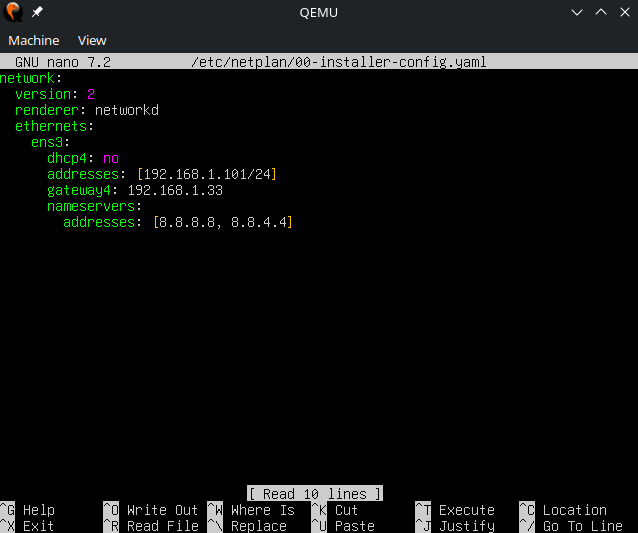
\includegraphics[width=0.7\textwidth]{1.png}
    \caption{Configuración de Netplan en la VM QEMU}
    \label{fig:netplan_vm}
\end{figure}
\newpage
\subsection{Configuración de QEMU para usar el bridge}

Archivo de script \texttt{qemuUS.sh}:

\begin{lstlisting}[language=bash, caption=Script para lanzar VM con QEMU usando br0]
sudo qemu-system-x86_64 \
  -enable-kvm \
  -m 4096 \
  -smp 2 \
  -cpu host \
  -hda /home/archi/Downloads/ubuntu-server.qcow2 \
  -boot d \
  -netdev bridge,id=net0,br=br0 \
  -device virtio-net-pci,netdev=net0 \
  -vga virtio
\end{lstlisting}

\textbf{Explicación:}
\begin{itemize}
    \item \texttt{-netdev bridge,id=net0,br=br0} conecta la VM al bridge creado.
    \item \texttt{-device virtio-net-pci,netdev=net0} proporciona la interfaz virtual en la VM.
\end{itemize}
\newpage
\subsection{Configuración persistente con systemd-networkd}

\textbf{Archivo \texttt{/etc/systemd/network/br0.netdev}:}
\begin{lstlisting}[language=bash]
[NetDev]
Name=br0
Kind=bridge
\end{lstlisting}

\textbf{Archivo \texttt{/etc/systemd/network/enp5s0.network}:}
\begin{lstlisting}[language=bash]
[Match]
Name=enp5s0

[Network]
Bridge=br0
\end{lstlisting}

\textbf{Archivo \texttt{/etc/systemd/network/br0.network}:}
\begin{lstlisting}[language=bash]
[Match]
Name=br0

[Network]
Address=192.168.1.33/24
Gateway=192.168.1.1
DNS=8.8.8.8
\end{lstlisting}

\textbf{Habilitar servicios:}
\begin{lstlisting}[language=bash]
sudo systemctl enable --now systemd-networkd
sudo systemctl enable --now systemd-resolved
\end{lstlisting}
\newpage
\section{Configuración de K3s}

\subsection{Instalación y configuración del nodo Master (VM)}

\textbf{Instalación de K3s en la VM Master:}

\begin{lstlisting}[language=bash]
curl -sfL https://get.k3s.io | sh -
sudo k3s kubectl get nodes
\end{lstlisting}

\textbf{Obtención del token para unir nodos:}

\begin{lstlisting}[language=bash]
sudo cat /var/lib/rancher/k3s/server/node-token
\end{lstlisting}

\subsection{Unión de la Raspberry Pi como nodo Agent (Slave)}

\textbf{Comando para unir la Raspberry al Master:}

\begin{lstlisting}[language=bash]
curl -sfL https://get.k3s.io | K3S_URL=https://192.168.1.101:6443 K3S_TOKEN=<TOKEN_DEL_MASTER> sh -
\end{lstlisting}

\textbf{Verificación de nodos en el Master:}

\begin{lstlisting}[language=bash]
sudo k3s kubectl get nodes
# Deberías ver algo así:
# NAME   STATUS   ROLES                  AGE   VERSION
# k3s    Ready    control-plane,master   42h   v1.33.5+k3s1
# raspberry Ready <none>                 5s    v1.33.5+k3s1
\end{lstlisting}
\newpage

\section{Instalación del Dashboard de Kubernetes}

\subsection{Despliegue del Dashboard}

\textbf{Aplicación del manifiesto oficial (v2.7.0) en el nodo Master:}

\begin{lstlisting}[language=bash]
sudo k3s kubectl apply -f https://raw.githubusercontent.com/kubernetes/dashboard/v2.7.0/aio/deploy/recommended.yaml
\end{lstlisting}

\textbf{Salida esperada:}
\begin{lstlisting}[language=bash]
namespace/kubernetes-dashboard created
serviceaccount/kubernetes-dashboard created
service/kubernetes-dashboard created
...
deployment.apps/dashboard-metrics-scraper created
\end{lstlisting}

\subsection{Creación del usuario administrador}

\textbf{Archivo \texttt{dashboard-admin.yaml}:}

\begin{lstlisting}[language=yaml]
apiVersion: v1
kind: ServiceAccount
metadata:
  name: admin-user
  namespace: kubernetes-dashboard
---
apiVersion: rbac.authorization.k8s.io/v1
kind: ClusterRoleBinding
metadata:
  name: admin-user
roleRef:
  apiGroup: rbac.authorization.k8s.io
  kind: ClusterRole
  name: cluster-admin
subjects:
- kind: ServiceAccount
  name: admin-user
  namespace: kubernetes-dashboard
\end{lstlisting}

\textbf{Aplicación del usuario administrador:}

\begin{lstlisting}[language=bash]
sudo k3s kubectl apply -f dashboard-admin.yaml
\end{lstlisting}

\subsection{Generación del token de acceso}

\textbf{Comando para generar el token del usuario admin:}

\begin{lstlisting}[language=bash]
sudo k3s kubectl -n kubernetes-dashboard create token admin-user
\end{lstlisting}

\textbf{El token generado se utiliza para acceder al Dashboard vía web.}

\subsection{Acceso al Dashboard}

\textbf{Inicio del proxy local:}

\begin{lstlisting}[language=bash]
sudo k3s kubectl proxy
\end{lstlisting}

\textbf{El Dashboard queda accesible en:}

\begin{lstlisting}[language=bash]
http://127.0.0.1:8001/api/v1/namespaces/kubernetes-dashboard/services/https:kubernetes-dashboard:/proxy/
\end{lstlisting}

\textbf{Notas importantes:}
\begin{itemize}
    \item Es recomendable usar la versión 2.7.0 del Dashboard si la última versión falla con error 404.
    \item El token generado debe mantenerse seguro, ya que proporciona permisos de administrador.
    \item Asegúrate de que el nodo Master esté activo y listo antes de aplicar el manifiesto del Dashboard.
\end{itemize}

\section{Conclusión}

La creación del bridge permite que la VM tenga acceso directo a la red local y a Internet, facilitando la instalación de K3s y la integración con la Raspberry Pi como nodo slave. Esta configuración garantiza conectividad estable y control centralizado mediante la VM.

\clearpage
\section{Bibliografía}
\begin{thebibliography}{9}
\bibitem{qemu_bridge}
QEMU Documentation, ``Networking with QEMU'', 2023. \url{https://www.qemu.org/docs/master/network/}
\bibitem{k3s}
Rancher Labs, ``K3s Lightweight Kubernetes'', 2023. \url{https://k3s.io/}
\bibitem{systemd_networkd}
Systemd Documentation, ``systemd-networkd'', 2023. \url{https://www.freedesktop.org/software/systemd/man/systemd-networkd.service.html}
\end{thebibliography}

\end{document}
